\subsubsection{Thiết kế xác thực và phân quyền}
\label{sec:auth-design}
Hệ thống tách ba câu hỏi: người gọi là ai (JWT), có vai trò nào (Role), và có quyền trên đối tượng cụ thể không (chủ đơn). User lưu email duy nhất, passwordHash, role và điểm; role mặc định CUSTOMER. API đăng ký công khai không nhận quyền BARISTA từ dữ liệu khách gửi. Tài khoản quầy được cấp qua quy trình quản trị dữ liệu.

\begin{table}[htbp]\centering\small
\begin{tabularx}{\linewidth}{|p{.31\linewidth}|X|}\hline
\textbf{Nhóm thao tác} & \textbf{Điều kiện backend}\\\hline
Menu, chi tiết; đăng ký/đăng nhập & Được truy cập không cần JWT; input đăng ký/đăng nhập vẫn qua DTO validation.\\\hline
Thông tin tài khoản hiện tại & JWT hợp lệ; danh tính lấy từ token đã xác minh và User trong database.\\\hline
Xem/tạo/hủy/thanh toán đơn cá nhân & JWT hợp lệ và điều kiện nghiệp vụ; khi thao tác trên đơn có sẵn phải kiểm userId là chủ đơn.\\\hline
Hàng đợi, cập nhật trạng thái và quyết định của quầy & JWT hợp lệ, role BARISTA và luật trạng thái/version/transaction tương ứng.\\\hline
Khách xem/rút yêu cầu đổi & JWT và chủ Order nguồn; không có quyền tự duyệt hoặc tự xác nhận hoàn khoản thu dư.\\\hline
IPN/Return từ VNPay & Dữ liệu giao thức được kiểm chữ ký và tham chiếu, không dùng JWT của khách làm chứng thực callback cổng.\\\hline
\end{tabularx}\caption{Điều kiện truy cập theo danh tính, vai trò và chủ thể dữ liệu}
\end{table}

Thiếu token, token không hợp lệ/hết hạn hoặc người dùng không còn tồn tại bị từ chối xác thực (401). Tài khoản đã xác thực nhưng không có vai trò staff bị từ chối quyền (403). Với API đọc/hủy đơn cá nhân, đơn không thuộc người gọi được trả như không tìm thấy (404). Các mã lỗi có phạm vi khác nhau; việc ẩn nút quầy trên frontend không thay thế kiểm tra backend.

\begin{figure}[htbp]\centering
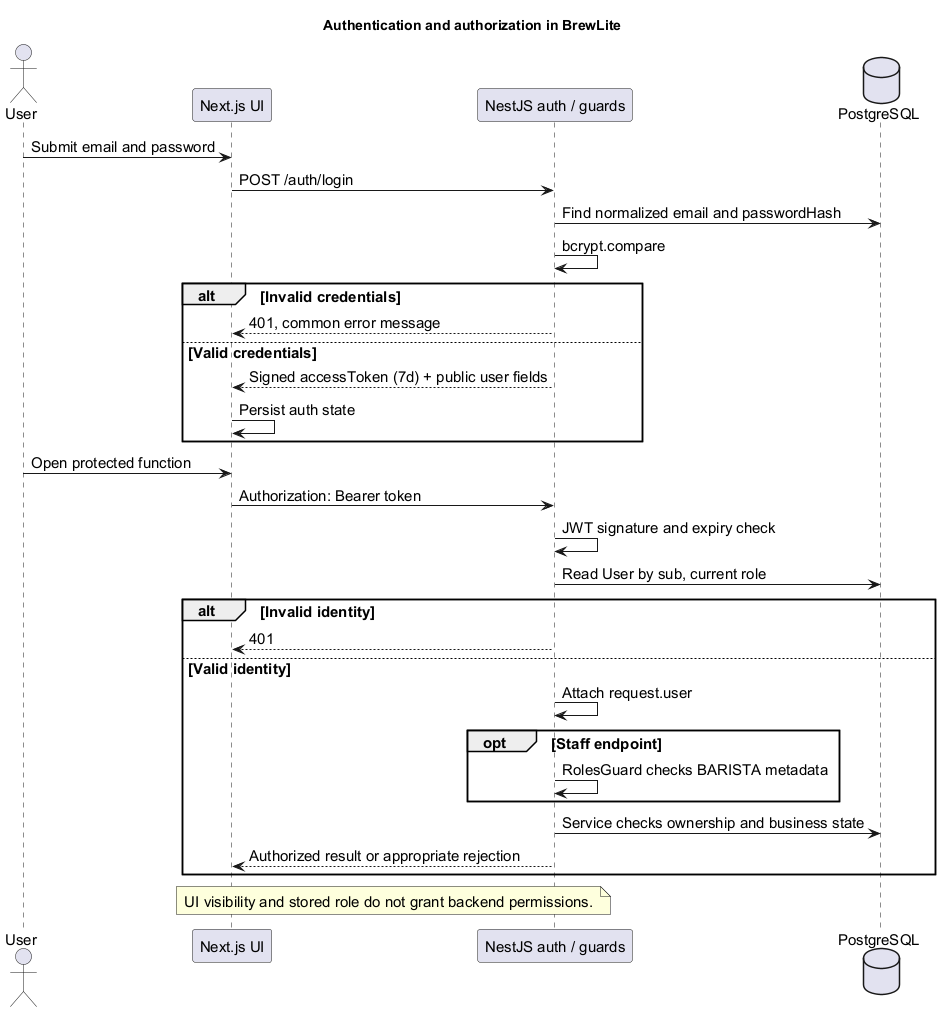
\includegraphics[width=\linewidth,height=.54\textheight,keepaspectratio]{assets/auth/auth-sequence.png}
\caption{Đăng nhập cấp token và chuỗi kiểm danh tính, vai trò, chủ đơn ở backend}
\end{figure}
